%\documentclass[a4paper,openright,14pt]{report}
%\usepackage[spanish]{babel}
%\selectlanguage{spanish}
%\usepackage[utf8]{inputenc}
%\usepackage{hyperref} %Para los enlaces
%\usepackage{multirow, array} % Para las tablas
%\usepackage{float}
%\usepackage{graphicx}

%%%%%%%%%%%%%%%%%%%%%%%%%%%%%%%%%%%%%%%%%%%%%%%%%%%%%%%%%%%%%%%%%%%%%%%%%%%%%
% Chapter 1: Introducción 
%%%%%%%%%%%%%%%%%%%%%%%%%%%%%%%%%%%%%%%%%%%%%%%%%%%%%%%%%%%%%%%%%%%%%%%%%%%%%%%

%---------------------------------------------------------------------------------
%\begin{document}
%\chapter{Introducción}\label{intro}

\section{Objetivos}\label{cap.1.1}
El objetivo de este trabajo de fin de grado (en adelante, TFG) es el desarrollo de una aplicación web para la gestión del escandallo, es decir, controlar el precio de producción de una receta. Para ello usaremos Cloud Servers, concretamente Google Cloud Platform, sin embargo, por algunas de las restricciones que mostraba, las cuales se describirán más adelante, se reorientó el TFG hacia otras plataformas como servicio (SaaS). Para su desarrollo usé la metodología de software ágil basada en el desarrollo dirigido por pruebas (TDD). Como framework, Sinatra (Ruby) para desarrollar la aplicación, integrar APIs de terceros, y hacer uso de varias nubes de producción a la vez y también herramientas de soporte para el desarrollo de software como son Github y Travis, entre otras.

\vspace*{0.2in}
\section{Antecedentes y estado actual del tema}\label{cap.1.2}
Los antecedentes y estudio de campo no sólo se centran en el tipo de aplicación que vamos a desarrollar, también tendremos en cuenta el entorno de producción, es decir, la nube donde estará disponible la aplicación web. Por lo tanto, tenemos dos puntos iniciales de estudio: 
\begin{itemize}
	\item Sobre la aplicación: 
	\begin{itemize}
		\item ¿Qué ofrece y por qué? 
		\item ¿Qué otras aplicaciones similares existen?
		\item Estudio del sector del mercado.
		\item Soporte y aspectos de la usabilidad.
	\end{itemize}

	\item Y respecto a la nube:
	\begin{itemize}
		\item ¿Cuál es la mejor nube que se adapte a nuestras necesidades?
		\item ¿Qué lenguajes y frameworks soporta?
		\item Período, costos, capacidad, etc.
	\end{itemize}
\end{itemize}

\vspace*{0.2in}
\begin{LARGE}
	\textbf {Aplicación}
\end{LARGE}

\vspace*{0.1in}
La finalidad de esta aplicación nace de la necesidad de optimizar los gastos, tanto en negocios de restauración como en los propios hogares. Hacer la comida controlando gastos es posible. En la actualidad existen en el mercado aplicaciones con esta idea, algunas de las mas destacadas son:
\begin{itemize}
	\item \href{https://recipecostcalculator.net/}{Recipe Cost Calculator}: Quizás sea la aplicación base como referencia, su fácil gestión y múltiples funciones la hace una herramienta útil y potente. Esta principalmente orientada a negocios.
	\item \href{http://www.recipe-costing.com/}{Recipe Costing}: Esta aplicación va más allá de las funcinalidades básicas, presenta extras como cálculos de menús, gestión de inventario, órdenes de compra a proveedores, etc.
	\item \href{http://developer.pearson.com/apis/pearson-kitchen-manager}{Pearson Kitchen Manager}: Se trata de una API, un banco de información que contiene más de 3000 mil recetas etiquetadas y con otra información como sus valores nutricionales.
	\item \href{https://itunes.apple.com/es/app/recipe-costing-calculator/id646877156?mt=8}{Recipe Costing Calculator}: Es más sencilla que las anteriores pero se trata de App disponible en iTunes. Las cosas más sencillas puden ser las más útiles, hay que tener en cuenta que un cocinero/a prefiere una tablet a un ordenador en la cocina.
\end{itemize}
La segmentación del mercado está orientado especialmente a negocios de restauración: comedores, restaurantes, bares, pastelerías, panaderías, etc. Por otro lado, existe otro sector que no se tiene tan en cuenta debido a que no genera tantos beneficios, se trata de los hogares. Las personas también pueden hacer uso de esta herramienta pues sus necesidades son las mismas pero a menor escala. En el próximo capítulo~\ref{chapter:dos}, se describe toda la funcionalidad de la aplicación, al igual que nos enseña como usarla y veremos las diferencias en la aplicación en función de a qué mercado está dirigido.\\

Por último, hay que tener en cuenta el soporte para la aplicación. Aprovechando la infraestructura y poder de Internet, la mejor opción es crear una aplicación web, que aunque en esta primera versión se diseñará de forma adaptativa, la idea es poder utilizarla en el futuro en dispositivos móviles y tablets. Además, se ha tenido en cuenta los aspectos de usabilidad durante su diseño.

\vspace*{0.3in}
\begin{LARGE}
	\textbf{{\huge Nube (cloud)}}
\end{LARGE}

\vspace*{0.1in}
Inicialmente la idea es trabajar en la \href{https://cloud.google.com/appengine/docs}{nube de Google}. Se trata de una plataforma como servicio (PaaS), la cual permite crear y mantener de forma sencilla una aplicación en la infraestructura de Google. Además permite una fácil escalabilidad de transeferencia de datos y almacenamiento gracias a sus módulos.\\

Empleando los conocimientos adquiridos durante los últimos cursos en Ruby y sus variedad de frameworks (Ruby on Rails, Padrino, Sinatra) lo usaré para crear la aplicación. Tras investigar y ver los servicios que ofrece Google App Engine (GAE) parece viable la puesta en marcha de la aplicación. GAE soporta cuatro lenguajes y sus correspondientes frameworks:
\begin{itemize}
	\item \href{https://cloud.google.com/appengine/docs/python/gettingstartedpython27/introduction}{Python} con webapp2 y Jinja2.
	\item \href{https://cloud.google.com/appengine/docs/java/gettingstarted/introduction}{Java} con maven.
	\item \href{https://cloud.google.com/appengine/docs/php/gettingstarted/introduction}{PHP} con Cloud SQL.
	\item \href{https://cloud.google.com/appengine/docs/go/gettingstarted/introduction}{Go} con el paquete html/plantilla. 
\end{itemize}

\begin{figure}[H]
	\centering
		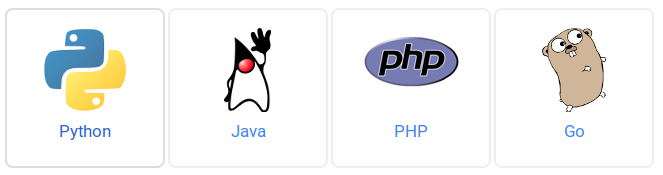
\includegraphics[width=10cm]{./images/lenguajes-GAE.png}
		\caption{Lenguajes soportados en GAE} \label{fig:lenguajes-GAE}
\end{figure}

Sin embargo, también es posible hacerlo funcionar en Ruby con la ayuda de java, juntos forman \href{http://jruby.org/}{JRuby}, el cual es una implementación 100\% del lenguaje Ruby. Además funciona como lenguaje embebido dentro de la máquina virtual de Java. Gracias a esta capa, podré programar en Ruby y Jruby establecerá una capa intermedia entre el código fuente en Ruby y el servidor en java. Para interactuar con la aplicación en la nube provee de una herramienta o kit, en este caso se trata de una gema llamada \href{https://rubygems.org/gems/google-appengine}{google-appengine}, sin embargo, la gema
dedicada a tal fin esta desfasada y el proyecto ha sido \href{https://code.google.com/p/appengine-jruby/}{archivado}.\\

Tras la incompatibilidad del proyecto de JRuby en GAE busco la opción más parecida posible que me ofrezca soporte, en este caso Google Cloud Platform. Tras investigar encuentro multitud de \href{https://cloud.google.com/launcher/explore}{lenguajes compatibles}, entre ellos Ruby, sin embargo, los servicios de esta nube son de pago y aunque existe una versión demo durante 60 días. Debido al tiempo que emplearía en el estudio, desarrollo y pruebas, este período puede resultar corto. Me pongo en contacto con el servicio de clientes y soporte de Google para bajar otras opciones, pero no ofrecen nada que me sea viable para desarrollar mi proyecto.\\

De esta forma se modifica el requisito inicial del TFG de usar los servicios de la nube de Google para encontrar y usar otros entornos de producción. La idea es intentar usar más de uno, demostrando la modularidad de la aplicación, esto significa que el código fuente de la aplicación debe ser único para las distintas nubes de producción. El siguiente paso es investigar las nubes que se ofertan. La siguiente tabla muestra un resumen:

\begin{table}[H]
	\centering
	\begin{tabular}{p{2cm} p{8cm}}
	\hline
	\textbf{Nube} & \textbf{Comentario} \\
	\hline \hline
	\href{https://cloud.google.com/free-trial/?hl=es&_ga=1.261030148.846668794.1427305506}{Google} & De pago. Prueba gratuita de 60 días. Multitud de servicios, distintos tipos de bbdd y soporta muchos \href{https://cloud.google.com/launcher/?hl=es}{lenguajes} y frameworks. \\
	\hline
	\cite{URL:Azure} & De pago. Prueba de 30 días. Soporta varios \href{https://tryappservice.azure.com/}{lenguajes}. \\
	\hline
	\href{https://c9.io/}{cloud9} & Se trata de un entorno de trabajo, una nube orientada al desarrollo, no es lo que buscamos. \\
	\hline
	\href{https://www.nitrous.io/}{nitrous} & Es similar a la anterior. Orientada al trabajo colaborativo en entornos de desarrollo. \\
	\hline
	\href{https://www.dotcloud.com/}{dotCloud} & Esta es una propuesta válida. Se trata de una nube de producción con servicios de pago y versión básica gratuita. Soporta varios \href{https://www.dotcloud.com/dev-center/guides}{lenguajes}. El uso de módulos como bbdd o rendimiento del servidor son de pago. \\
	\hline
	\href{https://www.heroku.com/}{Heroku} & Ideal para experimentar con aplicaciones en la nube en un módulo limitada. Su uso es ilimitado, pero tiene algunas \href{https://www.heroku.com/pricing}{condiciones}. Soporta varios \href{https://devcenter.heroku.com/categories/language-support}{lenguajes} y frameworks. \\
	\hline
	\href{https://www.openshift.com/}{OpenShift} & Es una alternativa muy interesante. Existe la opción de uso gratuito de hasta 3 aplicaciones. Soporta varios \href{https://www.openshift.com/promotions/try-openshift?sc_cid=70160000000UJArAAO&gclid=CMqo54DUy8cCFSMcwwodxLoGGQ}{lenguajes} y distintas versiones del mismo, así como 3 tipos de bbdd (PostgreSQL, MySQL y MongoDB) y los cartuchos (módulos) que añadamos son de pago. Podemos crear y subir nuestros propios cartuchos. \\
	\hline
	\href{https://www.appfog.com/}{appfog} & De pago con versión de prueba de 30 días. Soporta varios \href{https://www.ctl.io/appfog/}{lenguajes}. El enfoque de esta PaaS es facilitar el trabajo al equipo de desarrollo y que solo se centre en la aplicación y en los datos, mientras la nube gestionaría el resto. \\
	\hline
	\href{https://aws.amazon.com/es/?nc2=h_lg}{Amazon} & Presenta una gran infraestructura de servicios y recursos. Es de pago pero tiene una versión de prueba de 12 meses. Soporta varios lenguajes y dispone de multitud de productos orientados a distintos tipos de mercado. \\
	\hline
	\href{https://www.digitalocean.com/}{DigitalOcean} & Es de pago. Provee de infraestructura remota para que el desarrollador pueda lenvantor el tipo de servidor que desee. Soporta varios \href{https://www.digitalocean.com/community/}{lenguajes} y frameworks. \\
	\hline
	\href{http://www.cloud66.com/}{Cloud66} & Es de pago pero tiene un perídodo de 14 días de prueba. Esta orientada a mejora las aplicaciones que ya tenemos en otras nubes, en cuanto aspectos de crecimiento y seguridad. \\
	\hline
	\href{http://www.1and1.es/}{1 and 1} & Es de pago. Soporta diferentes lenguajes, frameworks y CMS. \\
	\hline
	\end{tabular}
	\caption{Production Clouds}
	\label{tabla:clouds}
\end{table}

Una vez analizadas se propone como entornos de producción las nubes Heroku y Openshift, de las cuales se entrará en detalle en el capítulo~\ref{chapter:tres}.

%----------------------------------------------------------------------------------

\vspace*{0.2in}
\section{Metodología de trabajo}\label{cap.1.3}

Durante la investigación y desarrollo de este proyecto se ha apostado por las metodologías ágiles, si bien no ha sido en un grupo de trabajo, se puede aplicar en lo que se refiere al análisis, al desarrollo y diseño de la aplicación y a las reuniones con el \emph{cliente}, cuyo rol lo asume el tutor junto con el de \emph{jefe de proyecto}. \\

Estos métodos están basados en el desarrollo iterativo e incremental, donde los requisitos y soluciones evolucionan mediante la colaboración de grupos. La idea es minimizar riesgos desarrollando software en períodos cortos. Este período se llama \textbf{iteración} cuya duración se define en función de los requisitos del proyecto, especialmente recursos de tiempo y humano. \\

\begin{figure}[H]
	\centering
	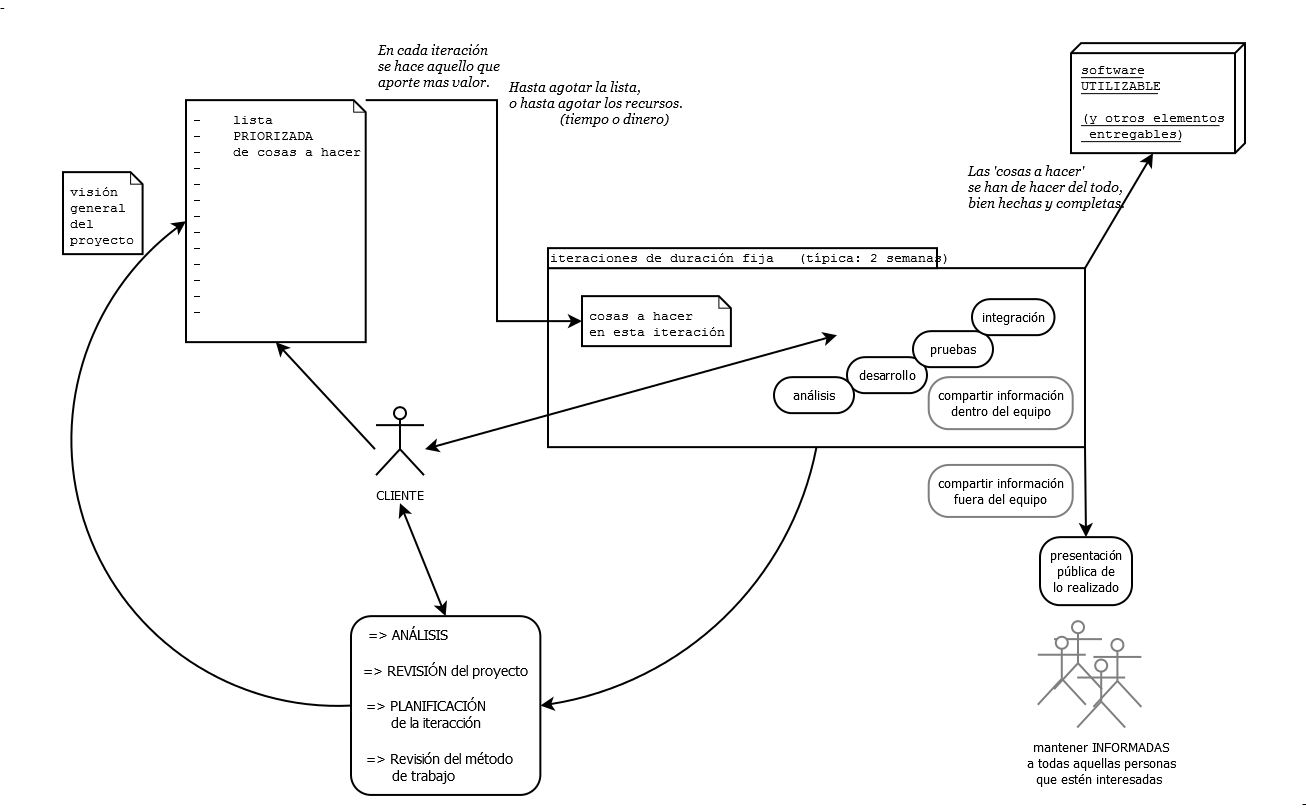
\includegraphics[width=14cm]{./images/metodologia-agil.png}
	\caption{Esquema de metodología ágil} \label{fig:metodologia}
\end{figure}

\vspace*{0.1in}
Cada iteración del ciclo de vida incluye:
\begin{itemize}
	\item Planificación: organización del trabajo durante una iteración. En este caso, la planificación corresponde con las tutorías y seguimiento semanal con el tutor.
	\item Análisis de requisitos: cada nueva funcionalidad o idea para la aplicación debe ser estudiada. Así, si por ejemplo, si quiero integrar una API debo considerar si es útil o no, si es compatible con los entornos de producción y con el lenguaje, documentarme para su integración en la aplicación, etc.
	\item Diseño: interfaz de la aplicación, características y aspectos de usabilidad.
	\item Codificación: corresponde por lo general a escribir código, aunque esto no se limita solo a realizar la propia aplicación, además se incluyen los tests y todos aquellos prototipos y pruebas durante la etapa de estudio de campo.
	\item Revisión: incluye superar los tests con éxito y la aceptación por parte del cliente.
	\item Documentación: para este trabajo en concreto, se realizó un diario semanal, cuya síntesis se engloba en este documento.
\end{itemize}

Durante este proyecto se ha seguido dicho ciclo de vida con especial importacia. He intentado adaptar la metodología Scrum a este trabajo, aunque no se ha tenido en cuenta  el aspecto de los roles. En Scrum se realizan entregas parciales y regulares del producto final. Scrum está especialmente indicado para proyectos en entornos complejos, donde se necesita obtener resultados pronto, donde los requisitos son cambiantes o poco definidos, donde la innovación, la competitividad, la flexibilidad y la productividad son fundamentales. \\

Cabe destacar dada la utilización del framework de Sintra, el uso inherente del modelo-vista-controlador (MVC) durante la etapa de diseño, desarrollo y pruebas. Se describirá detalladamente en el capítulo~\ref{chapter:cuatro} así como su uso para crear Chefmanagement.

%\end{document}


%---------------------------------------------------------------------------------
%Citando una entrada de memtfg.bib \cite{URL:GitHub}

%Incluyento una gráfica y referenciandola como Figura \ref{fig:prueba} y tambien un poco de código como Listado \ref{code:prueba}
